\part{Résultats et discussion}

\chapter{Des résultats prometteurs}

Pour construire notre indice global d’agentivité, calculé au niveau de chaque pièce, nous avons tout d'abord normalisé les mesures de chaque métrique linguistique afin qu’elles soient comprises entre 0 et 1. Nous avons ensuite additionné, pour une pièce considérée, le score de toutes les métriques calculées par statut (haut/bas) ou respectivement par genre (masculin/féminin), des personnages ayant prononcé les répliques concaténées, et sur la base desquelles chaque métrique avait été calculée dans la pièce en question. La somme obtenue correspond ainsi, pour chaque pièce, au score d’une  « méga-variable » calculée par statut (resp. par genre), et constituant la première ébauche de notre indice agentif. Ce score est compris entre 0 et 1.

Au total (en considérant toutes les pièces analysées dans notre corpus), nous disposons de 888 observations afin de tester l’association entre  « mégascore » agentif et statut des personnages, et de 891 observations s’agissant de l’association entre le mégascore agentif et le genre des personnages. 
A partir de tous ces points, nous tentons donc d’estimer la corrélation entre l'indice d’agentivité ainsi construit et la variable catégorielle \textit{statut} (resp. \textit{genre}), à l'aide de différents modèles de régression linéaire détaillés ci-après :

-Un modèle de régression simple calculant l’impact du Statut (resp. Genre) sur le mégascore agentif.

-Un modèle de régression logit calculant à l’inverse l’impact du mégascore agentif sur le Statut (resp. Genre) des personnages locuteurs.

A noter que pour l’analyse s’intéressant au statut, nous avons en réalité construit non pas deux mais quatre modèles de régression au total, en dupliquant chaque modèle selon que l’on prenait en compte, ou non, la direction de corrélation attendue (positive ou négative) pour chacune des métriques linguistiques avec le score agentif. On notera que les verbes sont comptés positivement ici, y compris les verbes modaux et l'usage de la modalité en général (en ce qu'elle reflète supposément une agentivité  « morale »), ce malgré l'ambiguïté mentionnée dans les sections correspondantes pour ces marqueurs. L'on considère en effet dans cette première ébauche que le verbe reste, intuitivement, un proto-marqueur agentif qu'il serait difficile d'ignorer, en sachant que si la direction s'avère contraire à celle prédite, cela ne devrait pas être suffisamment important pour affecter la direction du score global étant donnée la multitude d'autres métriques incluses dans son calcul. Et c'est en ce sens que nous conservons malgré tout un calcul plus  « grossier » du score agentif, qui somme simplement toutes les métriques dont on pense qu'elles ont avoir avec la notion d'agentivité, quelle que soit la direction de la corrélation postulée.
Nous avons également supprimé du calcul du score agentif, dans la seconde version des modèles, les métriques pour lesquelles la direction de corrélation demeurait trop ambigüe, à savoir : le nombre de parenthèses, points, virgules, points-virgules, deux points, guillemets, apostrophes, tirets et l'emploi du gérondif\footnote{Ces métriques n'ont d'ailleurs pas été mentionnées du tout, ou seulement très brièvement, dans le corps de ce mémoire. En guise de précision donc, les signes de ponctuation supprimés dans la seconde version des modèles étaient régulièrement associés à des traits de personnalité d'intérêt du \textit{Big Five} dans les études correspondantes parcourues, mais ce de façon contradictoire et \textit{a fortiori }non distinctive. Quant au gérondif, l'on avait supposé qu'il pourrait venir s'ajouter aux proxy téliques individuels - hors analyse compositionnelle, en ce qu'il dénoterait en l'occurrence un aspect atélique par la focalisation sur le déroulement de l'action qu'il sous-tend. Cela dit, cette interprétation demeurait très personnelle et incertaine, n'étant soutenue par aucune étude spécifique. Il est donc également supprimé du calcul du score dans la seconde version des modèles. On précisera enfin, au passage, que la suppression des métriques comptant le nombre de phrases et de mots prononcés dans le calcul de l'indice agentif ne change pas la significativité des résultats qui suivent, de sorte que cet indice ne se contente pas de révéler le fait qu'un maitre parle plus souvent, et/ou plus longtemps, que son serviteur dans la pièce, toutes les autres métriques incluses étant normalisées en fonction du nombre total de mots dans chacun des deux groupes de répliques précisément afin de prévenir ce biais.}.

Ce problème ne s’est pas posé concernant le genre, pour lequel nous n’avions pas de quoi supposer, \textit{a piriori}, une direction de corrélation précise pour chaque métrique de l’indice, par rapport au genre. Dans ce cas en effet, nous supposons simplement que le score agentif, même s'il comprend certaines métriques en réalité inversement corrélées à ce dernier et ayant donc un score plus faible quand ce degré d'agentivité augmente, devrait globalement corréler positivement avec le genre masculin, contrairement à celui féminin.

Concernant le statut des personnages tout d’abord, les résultats sont donc présentés ici respectivement sans et avec prise en compte des directions de corrélation propres à chaque métrique (à savoir que dans la seconde version de chacun des modèles, les métriques suivantes ont été comptées négativement au moment de calculer le mégascore agentif : ponctuation, ellipses, ratio du nombre de \textit{tokens} différents utilisés par rapport au nombre total de mots ou lemmes - deux versions d'une même métrique, indice de richesse lexicale, noms, articles, adverbes de manière, adverbes de doute, négations, présent, imparfait, indicatif, verbes statifs, copules, prépositions de manière, formalité, style  « dynamique »).

En moyenne, le mégascore agentif est de 23.5 pour les personnages de haut statut contre 22.5 pour ceux de bas statut (respectivement 7.35 contre 6.24 en prenant en compte les directions).

\begin{table}[ht]
\caption{Score agentif par statut - modèle 1}
\centering
\bigskip
\begin{tabular}{lS[table-format=2.1]S[table-format=1.3]}
    \hline
    Statut &  Moyenne & Ecart-type \\
    \hline
    Haut &  23.5 & 0.826 \\
    Bas &  22.5 & 1.22 \\
    \hline
\end{tabular}
 \label{Tab:moystatut}
\end{table}
\bigskip

\begin{table}[ht]
\caption{Score agentif par statut - modèle 2}
\centering
\bigskip
\begin{tabular}{lS[table-format=2.1]S[table-format=1.3]}
    \hline
    Statut &  Moyenne & Ecart-type \\
    \hline
    Haut &  7.35 & 0.940 \\
    Bas &  6.24 & 1.05 \\
    \hline
\end{tabular}
 \label{Tab:moy_statut}
\end{table}
\bigskip

Aussi, un t.test nous révèle que la différence de moyenne du mégascore agentif entre ces deux statuts est chaque fois significative (p < 0.001). 

En appliquant le modèle de régression linéaire simple suivant : 

\begin{equation}
\text{Score} \, \text{agentif} \, \sim \, \text{Statut}
\end{equation}

On trouve de façon cohérente qu’il existe une association linéaire significative entre le mégascore agentif et la variable catégorique \textit{statut}, ce avec et sans prise en compte des directions de corrélation individuelles (p < 0.001). 

D’après le premier modèle, le fait de passer de la catégorie  « bas » à  « haut » statut, toutes choses égales par ailleurs, augmente la valeur moyenne du score agentif de 1.01, contre 1.11 dans le second modèle.

Le $R^2$ pour chacun des deux modèles est de 0.19 et 0.24 respectivement, avec un sigma (écart-type du terme d’erreur) de 1.04 et 1. Le second modèle explique donc une plus grande proportion de la variance du score agentif, et génère des prédictions plus proches des points de données réels (sigma plus faible). Il peut ainsi être considéré comme ayant une meilleure adéquation aussi bien en termes de $R^2$ que de minimisation des erreurs de prédiction. 

Puisqu’il n’était pas aisé de savoir si l’on s’attendait à ce que le statut permette de prédire le langage utilisé dans la pièce, ou bien plutôt à ce que l’utilisation d’un certain langage prédise le statut des personnages, nous avons également analysé le modèle de régression logistique suivant : 

\begin{equation}
\text{Statut} \, \sim \, \text{Score} \, \text{agentif}
\end{equation}

Là encore, l’association est chaque fois très significative (p < 0.001), la seconde version du modèle (avec prise en compte des directions individuelles) présentant de façon cohérente un meilleur « fit » que la première (déviance résiduelle et AIC plus faible), ainsi qu'un coefficient de score agentif un peu plus élevé. 

Exprimé en ratio de vraisemblance (et non plus en logarithme de ce dernier), le premier modèle indique que pour chaque augmentation d’une unité du score agentif des répliques considérées, les chances que leurs locuteurs soient de haut statut sont 2.8 fois plus élevées, toutes choses égales par ailleurs (l’intervalle de confiance à 95\% associé étant : [2.29, 3.53]). Le second modèle (avec prise en compte des directions individuelles) présente quant à lui un odds-ratio de 3.03 ([2.49, 3.75]).

S’agissant des modèles logistiques, nous avons encore testé leurs performances prédictives au moyen d’une validation croisée dix fois. La précision de chacun des modèles (sans et avec prise en compte des direction de corrélation respectivement) est de 75\% et 79\% respectivement, leur sensibilité de 78\% et 77\%, et ainsi leur F1-score de 77\% et 78\%. Si le second modèle est légèrement plus précis que le premier (relativement moins de faux positifs), leurs performances prédictives globales sont donc équivalentes.

\begin{table}[ht]
  	\caption{Résultats de l'évaluation des modèles logistiques relatifs au statut en validation croisée}
		\centering % Centre the table on the slide
		\begin{tabular}{l c c c c c}
			\toprule
    			 & precision & recall & f1-score \\
			\toprule
			Modèle 1 & 0.754 & 0.782 & 0.768 \\
			\midrule
			Modèle 2 & 0.786 & 0.774 & 0.780 \\
			\bottomrule
		\end{tabular}
            \label{Tab:logit_statut}
	\end{table} 

Concernant le genre des personnages cette fois, pour lequel nous avons systématiquement conservé toutes les métriques sans duplication des modèles, on trouve qu’en moyenne, le mégascore agentif est de 29 pour les personnages féminins contre 29.1 pour les locuteurs masculins. Un t.test nous confirme que cette différence de moyenne du mégascore agentif entre les deux genres n’est pas du tout significative (p = 0.9921). 


\begin{table}[ht]
\caption{Score agentif par genre}
\centering
\bigskip
\begin{tabular}{lS[table-format=2.1]S[table-format=1.3]}
    \hline
    Genre &  Moyenne & Ecart-type \\
    \hline
    Masculin &  29.1 & 0.830 \\
    Féminin &  29.0 & 1.06 \\
    \hline
\end{tabular}
 \label{Tab:moy_genre}
\end{table}
\bigskip

En appliquant le modèle de régression linéaire simple suivant : 

\begin{equation}
\text{Score} \, \text{agentif} \, \sim \, \text{Genre}
\end{equation}

On trouve qu’il existe une association linéaire faiblement significative (p = 0.0159) entre ces deux variables que sont le mégascore agentif et genre du personnage. 

Le fait de passer de la catégorie « féminin » à « masculin » augmente plus précisément la valeur moyenne du score agentif de 0.15, toutes choses égales par ailleurs.

Le $R^2$ du modèle est de 0.007, et son sigma de 0.95. Cela suggère que le genre, en tant que seul prédicteur, n'explique pas une grande partie de la variabilité du mégascore agentif. Sa significativité pratique serait donc limitée. Les prédictions du modèle sont du reste relativement proches des points de données réels (sigma faible).

Pour les mêmes raisons que précédemment, nous avons également analysé le modèle de régression logistique suivant : 

\begin{equation}
\text{Genre} \, \sim \, \text{Score} \, \text{agentif}
\end{equation}

Là encore, l’association est faiblement significative (p = 0.0374).

Aussi, le modèle indique que pour chaque augmentation d’une unité du score agentif des répliques considérées, les chances que leurs locuteurs soient des personnages masculins sont 1.2 fois plus élevées, toutes choses égales par ailleurs (l’intervalle de confiance à 95\% associé étant : [1.01, 1.45]). 

Nous avons à nouveau testé ses performances prédictives au moyen d’une validation croisée dix fois. La précision du modèle est de 54\%, sa sensibilité de 52\%, et ainsi son F1-score de 53\%. Ce modèle est donc, logiquement, très peu performant lorsqu’il s’agit de prédire le genre du personnage locuteur, sur la base du mégascore agentif seul.

\begin{table}[ht]
\caption{Résultats de l'évaluation du modèle logistique relatif au genre en validation croisée}
		\centering % Centre the table on the slide
		\begin{tabular}{l c c c c c}
			\toprule
    			 & precision & recall & f1-score \\
			\toprule
			     & 0.539 & 0.512 & 0.529 \\
			\bottomrule
		\end{tabular}
            \label{Tab:logit_genre}
	\end{table} 

\bigskip
Ces résultats constituent donc une première confirmation de nos intuitions théoriques, à savoir que le niveau d'agentivité d'un personnage, tel que nous l'avons défini théoriquement et sur la base d'une validation interne à la pièce (c'est-à-dire a priori informés par le statut du personnage), semble être identifiable de manière relativement systématique par un ensemble de marqueurs linguistiques au niveau agrégé. 

Il est également rassurant que la seconde version de notre modèle linéaire simple s’attachant à expliquer le mégascore agentif par le statut du personnage se révèle globalement plus performant que la première. A savoir que la prise en compte des directions de corrélation propre à chaque marqueur linguistique rend de fait le niveau d’agentivité des locuteurs (approximé par leur statut) plus « capable » d’expliquer leur mégascore agentif, ainsi calculé.

Néanmoins, la première tentative de validation externe de notre indice agentif global, au moyen du genre des personnages, est pour sa part peu concluante. De fait, l’association entre genre et mégascore agentif n’est que très faiblement significative, et les performances prédictives d’un modèle de régression logistique tentant d’expliquer ledit mégascore par le genre des locuteurs sont à peine supérieures à celles qu’obtiendrait un modèle de classification aléatoire. 

Cela étant, la notion de genre ne se limite pas à l’agentivité, et est susceptible de charrier un certain nombre d’autres dimensions qui pourraient précisément interférer avec le degré d’agentivité d’un individu au moment de façonner son langage. Il n’est donc pas étonnant que la corrélation soit moins évidente que pour le statut. Ce d'autant plus que, n'ayant pas eu le temps de nous plonger dans la littérature s'intéressant aux associations préférentielles entre genre et langage, nous n'avons pas entrepris d'affiner le calcul de notre indice par la prise en compte de la direction de corrélation précise attendue pour chaque métrique prise isolément (et il semblait peu justifié, à ce stade, de simplement répliquer les directions de corrélation prédites pour le statut et non pour le genre spécifiquement). Aussi, on notera que la direction globale prédite est quant à elle respectée, à savoir que l’indice agentif est bien préférentiellement associé au genre masculin, bien que cette préférence soit légère, par rapport à celui féminin.

\chapter{Discussion}

\section{Limites de la présente recherche}

Notre étude, très exploratoire, connait bien entendu certaines limites. 

Tout d’abord, un certain nombre de travaux sur lesquels nous nous appuyons afin de définir, \textit{a priori}, nos marqueurs linguistiques agentifs ne triangulent pas les données en faisant notamment appel, outre l'analyse de corpus par  « lecture distante », à des expériences psycholinguistiques. Certains marqueurs sont donc étiquetés agentifs sur la base de la seule appréciation subjective de l’auteur, et certains résultats sont d’ailleurs en partie mis en cause par des études contradictoires (pour la modalité notamment). 

Aussi, toutes ces études valent pour l’anglais et non le français. Pour autant, notre recherche s’intéressant en priorité à des marqueurs  « structurels » (c.a.d. aux niveaux grammatical et syntaxique) relativement simples, la transposition des conclusions au français ne nous semblait pas déraisonnable (la présence d’un objet grammatical par exemple, semble devoir produire un effet relativement similaire quelle que soit la langue considérée, d’autant plus entre des locuteurs appartenant à des sociétés culturellement proches comme le sont les Etats-Unis et la France). Nous sommes toutefois conscients qu'il existe des différences notables entre ces deux langues, s’agissant notamment du cadrage dit  « satellitaire » pour l'anglais et  « verbal » pour le français. En effet, l’on distingue depuis Talmy\footnote{\cite{talmy_path_1991}} deux grands types de langues : celles dites  « encadrées par le verbe », où l'emplacement et le mouvement sont encodés par le verbe principal d'une clause, une adjonction facultative se chargeant alors d’encoder la manière dont se déroule l’évènement  ; et celles à cadre  « satellitaire », où la localisation et le mouvement sont encodés par un élément associé au verbe, laissant le verbe libre d’encoder la manière. Aussi, cette typologie binaire traditionnelle en linguistique, entre  « chemin » et  « manière », est directement liée à la notion de télicité, une clause télique s’intéressant par définition davantage à la direction de l’évènement (sa finalité) qu’à la manière dont il s’est déroulé. Notre marqueur télique, défini de manière compositionnelle et sur la base d’études anglophones, s’avère donc très incertain, ce d’autant plus qu’il se fonde également sur des choix personnels. En particulier, l’analyse des prépositions pour décider de la télicité d’une clause (selon qu’elles soient  « directionnelles » -  « jusque »,  « jusqu' »,  « vers » – ou indiquant une manière de faire –  « sans »,  « avec »,  « par ») pourrait ne pas être pertinente s’agissant du français (bien que certaines études aient depuis contesté la validité de cette typologie binaire entre deux cadrages linguistiques du  « chemin » et de la  « manière »\footnote{\cite{egan_manner_2015}}). C’est pour cette raison que nous avons intégré à l’analyse le calcul isolé de proxy téliques plus  « grossiers », à savoir le temps du discours (parfait ou imparfait) et l’individuation de l’objet grammatical (présence d’un article défini, d’un déterminant possessif, démonstratif, numéral etc), calculés séparément de cette métrique compositionnelle.

La confection des listes d’adverbes pose également la question de leur solidité. Si les adverbes français exprimant une intention, un doute, ou une affirmation semblent \textit{a priori} exister en nombre limité, et que ces derniers ont été identifiés en prenant soin de recouper plusieurs grammaires françaises officielles, ces métriques doivent être interprétées avec précaution. Elles reposent en effet sur des choix personnels, et se placent à un niveau d’analyse sémantique qui reste soumis au risque de variation historique quant au sens et à la fréquence d’utilisation des mots considérés, variation pouvant être soutenue par des phénomènes de transmission culturelle non signifiants pour notre étude. Le noème d’ « intentionnalité » pourrait en outre être exprimé par différents éléments lexicaux selon les époques, selon un processus de glissement similaire à celui qui semble s’opérer entre verbes modaux et semi-modaux ce dernier siècle. L’augmentation de l’utilisation d’adverbes intentionnels ne saurait donc renseigner que de façon très partielle l’évolution de l’expression de l’intentionnalité, en général, à travers le temps. 

Enfin, en l’absence de validation externe, nos modèles d’analyse ne disent pour l’instant rien de la spécificité de notre indice agentif global, qui pourrait tout autant corréler avec le niveau de communion des personnages, par exemple.

\section{Analyses successives}

Etant donnée l’échec de la validation externe de notre indice par le genre des personnages, nous ne pouvons en effet pas encore être certains de son caractère distinctif au moment d’estimer le niveau d’agentivité d’un locuteur. Il faudrait encore étudier, en parallèle, les marqueurs d'extraversion et d'agréabilité, qui correspondent pour rappel aux deux traits de personnalité du modèle des \textit{Big 5} les plus directement corrélés à l’agentivité et à la communion respectivement. Pour que notre indice agentif soit spécifique, il faudrait alors que le mégascore d’extraversion ainsi obtenu soit significativement et positivement corrélé au statut des personnages, et que celui d’agréabilité soit à l’inverse non significativement corrélé au statut (ou même négativement corrélé à ce dernier, bien que l’agentivité et la communion soient \textit{a priori }orthogonales).

Nous avons pour ce faire déjà identifié les éléments linguistiques préférentiellement associés à l’extraversion (et dans une moindre mesure à la conscienciosité), et à l’agréabilité (et dans une moindre mesure à l’ouverture). Cette analyse pourrait être complétée par un usage plus global du LIWC, qui sert de support à la plupart des études s’intéressant au lien entre traits de personnalité et langage, en incluant ses composants sémantiques (qui n’ont pas été listés dans le tableau de la section \textit{III. 4. Le langage de la personnalité : indices d’extraversion et d’agréabilité} étant donnée la focalisation  « structurelle » de ce mémoire).

A titre subsidiaire, il serait également intéressant d’estimer l'interaction entre le statut et le genre des personnages au moment d’expliquer leur score agentif. Cette analyse n’a pu être menée ici car elle supposait de faier tourner notre code à nouveau (le temps de calcul étant conséquent), en calculant les métriques par personnage, et non plus sur leurs répliques concaténées. En effet, bien que le genre ne soit pas un prédicteur significatif de l’agentivité en tant que tel, il se pourrait que le fait d’être un homme exacerbe l’effet du statut sur le mégascore agentif.

Si tant est que notre indice global agentif soit distinctif, une analyse ultérieure consisterait à analyser plus finement l'importance relative de chaque métrique qui compose cet indice global, prise individuellement et/ou en les regroupant en sous-catégories selon certains critères tels que le niveau d'analyse auquel se situe la métrique (global, lexical, syntaxique, aspectuel etc.) – autant de regroupements qui permettraient de conserver suffisamment de puissance statistique tout en mettant en lumière les dimensions linguistiques les plus significatives au moment de prédire l’agentivité d’un texte. Nous pourrions alors affiner notre indice en lui ôtant les métriques s’avérant en réalité non significativement corrélées, prises individuellement, au statut des personnages, et de là le rendre potentiellement plus performant encore dans la reconnaissance de l’agentivité d’un locuteur.

Enfin, l’objectif ultime de cette étude est diachronique : il s’agit de tester l’hypothèse d’une corrélation positive entre niveau d’agentivité et niveau de ressources dans une société donnée, sur la base d’un paradigme évolutionnaire. Cela nécessiterait de construire un modèle de régression prédisant le niveau d’agentivité global d’un corpus de pièces, tel qu’estimé par l’indice agentif cette fois calculé sur l’ensemble des répliques, à partir d’un indicateur de développement économique (principalement le PIB par habitant et/ou le taux d'urbanisation), ce pour une société donnée et sur plusieurs fenêtres temporelles, en incluant potentiellement l’auteur de la pièce en tant qu’effet aléatoire\footnote{Pour une référence méthodologique qui s’appuie sur le même corpus de théâtre que celui utilisé ici : \cite{baumard_cultural_2022}}. Nous supposons qu’une association linéaire significative existe entre de tels indicateurs et le mégascore agentif des pièces étudiées, ce sur la base des observations recueillies à différentes périodes. En considérant que le niveau de ressources global augmente linéairement depuis 1600 au moins, nous nous attendons plus précisément à ce que le mégascore agentif des pièces augmente avec le temps, sur cette période du moins. Aussi, une analyse à l’échelle des personnages de la pièce, en distinguant à nouveau entre  « haut » et  « bas » statut, pourrait nous permettre de comprendre la façon dont ce score augmente : la différence entre les scores agentifs des personnages  « haut » et  « bas » statut se creuse-t-elle ? Ou bien tous les personnages deviennent-ils plus agentifs ? Conformément à notre paradigme évolutionnaire, l’on s’attendrait à ce que tous les personnages, quel que soit leur statut dans la pièce, s’expriment de manière plus agentive avec le temps. Un tel résultat serait d’ailleurs cohérent avec la théorie littéraire qui note souvent l’émergence d’une certaine porosité entre les rôles de maitres et de serviteurs au théâtre à partir du XVIII\ieme ~siècle, à l’image des pièces de Marivaux. 

Sur ce point, on s’attendrait ainsi à ce que l’ajout d’une variable d’interaction entre l’année de publication de la pièce et le statut des personnages dans nos précédents modèles de régression révèle un affaiblissement de l’association linéaire entre statut et indice agentif avec le temps (à savoir une interaction significativement négative entre le statut « bas » et l’année de publication), ce à mesure que les serviteurs deviennent supposément plus agentifs, jusqu’à emprunter le rôle, et ainsi peut être le langage, de leurs maitres. 

Néanmoins, ne disposant pour ce corpus que de 156 années de publication distinctes, nous ne bénéficiions pas d’une puissance statistique suffisante pour inclure une telle interaction \textit{per se}. Alternativement, nous pouvons simplement constater que la différence entre le score agentif des personnages « haut » et « bas » statut semble en effet varier avec la date de publication de l'oeuvre : 

\begin{figure}[!ht]
    \centering
    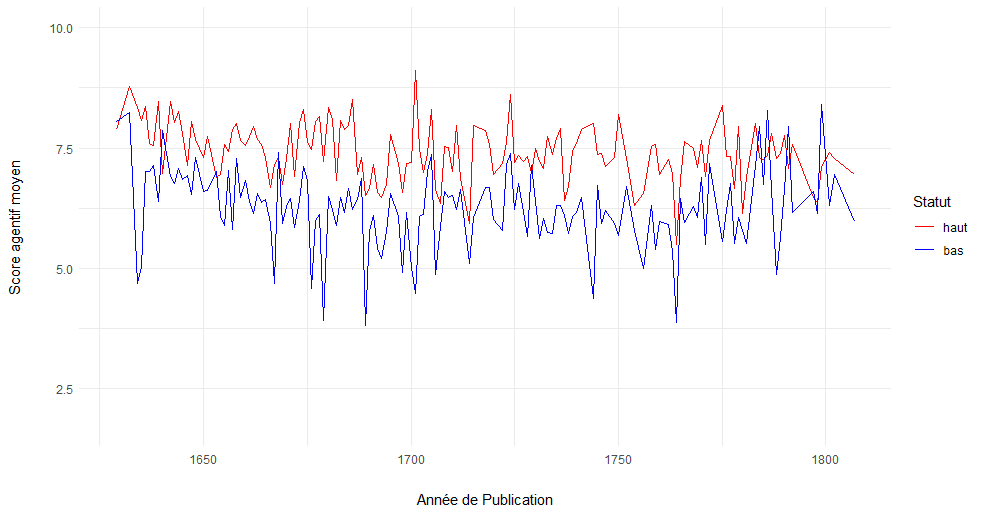
\includegraphics[width=16cm]{img/score_statut_par_annee_publication.png}
    \caption{Evolution du score agentif moyen des personnages haut et bas statut, selon l'année de publication}
    \label{score_statut_par_annee_publication}
\end{figure}

Nous avons ici réduit la période d’analyse pour ne s’intéresser qu’à l’intervalle de temps [1629-1807]. Les valeurs étant beaucoup plus espacées et extrêmes à partir de 1808, elles risquaient en effet d’influencer les résultats de façon disproportionnée. En outre, l'on précise que le score agentif analysé ci-après est celui calculé en prenant en compte la direction de corrélation prédite pour chaque métrique prise isolément (version 2 des modèles liés au statut).

De là, un modèle linéaire hiérarchique ou « à effets mixtes » incluant l'année comme intercept aléatoire permettait une première estimation de la façon dont l'effet du statut varie d'une année à l'autre. Plus précisément, en calculant la corrélation intraclasse (ICC), il apparait qu'environ 10\% de la variabilité totale du score agentif est attribuable aux différences entre les années sur la période 1629-1807.

En s’essayant à un premier regroupement des années de publication au sein de deux intervalles distincts ([1629-1699] et [1700-1807]), correspondant approximativement aux deux siècles d’analyse, et pour lesquels le nombre d’observations était globalement similaire (respectivement 450 et 414), l’on a également pu comparer les coefficients obtenus par notre modèle linéaire simple précédent (expliquant le score agentif par le statut des personnages) entre ces deux sous-périodes. L’on observe que la corrélation négative significative (p < 0.001) entre un statut « bas » et le score agentif diminue d’un intervalle à l’autre (passant de -1.163 sur la période 1629-1699 à -1.097 sur 1700-1807), ce qui est cohérent avec nos prédictions.

Malgré les limites de la présente étude, et précisément contre ces limites-mêmes concernant l’élaboration de certaines métriques individuelles, il semble donc que la conduite d’analyses successives soit justifiée (en premier lieu la détermination du caractère distinctif de notre indice). Notre indice agentif global est en effet significativement et très fortement corrélé à l’appartenance des personnages locuteurs à un « haut » statut, relativement aux personnages de  « bas » statut, et cela n'est pas simplement lié à une différence dans la longueur ou la fréquence des répliques entre ces deux types de personnages, mais bien à des marqueurs linguistiques plus fins. Il apparait même que l’on puisse déjà discerner des variations diachroniques dans cette association, bien que leur significativité, ainsi que leur corrélation avec le niveau de ressources environnant, reste encore à prouver.  